\section{Generating an Initial Guess: Matrix Pencil Method}
\label{sec:mpm}
In order for \ac{NLP} to perform effectively, a large amount of \textit{a
priori} information is typically required, in the form of an initial guess
$\bthzero$. Here, a description of one such approach to achieve this is presented blah blah blah...

\subsection{1D Matrix Pencil Method}
The \ac{MPM}, developed by Hua and Sarkar\cite{Hua1990,Hua1990b,Hua1991}, provides a
route to extracting the signal poles of a \ac{1D} dataset, based on the
assumption that the number or oscillators $M$ is known.

\subsubsection{Noiseless data}
To motivate how it
works, first consider a dataset which is devoid of noise, such that it is of
the form $\bXth$, given in Equation \ref{eq:x}, with $D=1$:
\begin{equation}
        \bX \left(\bth\right) \left[\none\right] =
            \sum_{m=0}^{M-1}
            \underbrace{
                \bdam \exp\left(
                    \iu \bdphim
                \right)
            \vphantom{
                \exp\left(
                    \left[ 2 \pi \iu \left(\bdfonem - \foff\right) - \bdetaonem\right] \none \Dtone
                \right)
            }}
            _{\bdalpham}
            \underbrace{
                \exp\left(
                    \left[ 2 \pi \iu \left(\bdfonem - \foff\right) - \bdetaonem\right] \none \Dtone
                \right)
            }_{\bdzonem^{\none}}.
            \label{eq:x1D}
\end{equation}
Consider the Hankel matrix $\HX \in \mathbb{C}^{(\None - \Lone) \times (\Lone + 1)}$:
\begin{equation}
    \HX =
    \begin{bmatrix}
        \bX[0] & \bX[1] & \cdots & \bX\left[\Lone\right] \\
        \bX[1] & \bX[2] & \cdots & \bX\left[\Lone+1\right] \\
        \vdots & \vdots & \ddots & \vdots\\
        \bX[\None-\Lone-1] & \bX[\None-\Lone] & \cdots & \bX[\None-1]\\
    \end{bmatrix}.
\end{equation}
This matrix comprises windowed segments of the FID, with each row comprising
the segment shifted to the right by one point relative to the row above. $\Lone
\in \mathbb{N}$ is the \emph{pencil parameter}, which dictates the size of each window
Define the two matrices $\HXone$ and $\HXtwo$, formed by the removal
of the last or first column of $\HX$, respectively:
\begin{subequations}
   \begin{gather}
        \HXone =
        \begin{bmatrix}
            \bX[0] & \bX[1] & \cdots & \bX\left[\Lone-1\right] \\
            \bX[1] & \bX[2] & \cdots & \bX\left[\Lone\right] \\
            \vdots & \vdots & \ddots & \vdots\\
            \bX[\None-\Lone-1] & \bX[\None-\Lone] & \cdots & \bX[\None-2]\\
        \end{bmatrix}, \\
        \HXtwo =
        \begin{bmatrix}
            \bX[1] & \bX[2] & \cdots & \bX\left[\Lone\right] \\
            \bX[2] & \bX[3] & \cdots & \bX\left[\Lone+1\right] \\
            \vdots & \vdots & \ddots & \vdots\\
            \bX[\None-\Lone] & \bX[\None-\Lone+1] & \cdots & \bX[\None-1]\\
        \end{bmatrix}.
   \end{gather}
\end{subequations}
These matrices can be deconstructed into the following forms involving matrices
containing the $M$ signal poles and complex amplitudes that the data comprises:
\begin{subequations}
   \begin{gather}
       \HXone = \symbf{Z}_{\text{L}} \symbf{A} \symbf{Z}_{\text{R}},\\
       \HXtwo = \symbf{Z}_{\text{L}} \symbf{A} \symbf{Z}_{\text{D}} \symbf{Z}_{\text{R}},\\
       \mathbb{C}^{\left(\None - \Lone\right) \times M} \ni
       \symbf{Z}_{\text{L}} =
       \begin{bmatrix}
           \symbf{1} &
           \bdzone &
           {\bdzone}^2 &
           \cdots &
            {\bdzone}^{\None-\Lone-1}
        \end{bmatrix}\T,\\
        \mathbb{C}^{M \times \Lone} \ni
        \symbf{Z}_{\text{R}} =
           \begin{bmatrix}
               \symbf{1} & \bdzone & {\bdzone}^{2} & \cdots & {\bdzone}^{\Lone-1}
           \end{bmatrix} ,\\
        \mathbb{C}^{M \times M} \ni
        \symbf{Z}_{\text{D}} = \diag\left(\bdzone\right), \label{eq:ZD}\\
        \mathbb{C}^{M \times M} \ni
        \symbf{A} = \diag\left(\symbf{\alpha}\right).\label{eq:A}
   \end{gather}
    \label{eq:HX-decomp}
\end{subequations}

\note{Description of what a matrix pencil is}
The matrix pencil $\HXtwo - \lambda\HXone, \lambda \in \mathbb{C}$ can
therefore be expressed as
\begin{equation}
    \HXtwo - \lambda \HXone = \symbf{Z}_{\text{L}} \symbf{A} \left(
        \symbf{Z}_{\text{D}} - \lambda \symbf{I}_M
    \right) \symbf{Z}_{\text{R}},
\end{equation}
where $\symbf{I}_M \in \mathbb{C}^{M \times M}$ is the identity matrix.
Assuming that the following condition is met:
\begin{equation}
    M \leq \Lone \leq \None - M,\label{eq:pencil_condition}
\end{equation}
the rank of the matrix pencil will be $M$. Equation \ref{eq:pencil_condition}
must be obeyed to ensure that both the number of rows and columns of the matrix
pencil are at least $M$. Now consider the case when the scalar $\lambda$ is
equal to one of the signal poles i.e.  $\lambda = \symbf{z}[m]\ \forall m \in
\lbrace 0, \cdots, M-1 \rbrace$. The element $\left(\symbf{Z}_{\text{D}} -
\lambda \symbf{I}_M\right) [m, m]$ will be set to $0$, which will lead to the
determinant of the matrix pencil being $0$. The eigenvalues of the matrix
pencil are the solution of the so-called \emph{generalised eigenvalue problem},
and are defined as\cite[Section 7.7]{Golub2013}
\begin{equation}
    \symbf{z} = \left\lbrace
        z \in \mathbb{C} : \det\left(\HXtwo - z \HXone\right) = 0
    \right\rbrace
\end{equation}
One means of finding the signal poles is by finding the eigenvalues of the
matrix $\HXone^+ \HXtwo^{\vphantom{+}}$. Deriving the corresponding complex
amplitudes can then be achieved by solving the set of linear equations
\begin{equation}
    \symbf{X} =
    \begin{bmatrix}
        \symbf{1} &
        {\bdzone} &
        {\bdzone}^2 &
        \cdots &
        {\bdzone}^{\None - 1}
    \end{bmatrix}\T
    \symbf{\alpha} \equiv \symbf{Z}^{(1)} \bdalpha \implies
    \symbf{\alpha} = \symbf{Z}^+ \symbf{X}.
\end{equation}
Extraction of the amplitudes, phases, frequencies, and damping factors from the
signal poles and complex amplitudes can then take place:
\begin{subequations}
    \begin{gather}
        \symbf{a} = \left \lvert \symbf{\alpha} \right \rvert,\\
        \symbf{\phi} = \arctan \left(\frac{\Im (\alpha)}{\Re(\alpha)}\right),\\
        \symbf{f}^{(1)} = \frac{\fswone}{2 \pi} \Im\left(\ln \bdzone \right) + \foff, \\
        \symbf{\eta}^{(1)} = -\fswone \Re\left(\ln \bdzone\right).
    \end{gather}
\end{subequations}

\subsubsection{Noisy data}
The presence of noise in the signal $\bY$ complicates the process of
determining the $M$ signal poles, as $\HY$ ($\HX$'s equivalent with elements
replaced by the noisy data) is likely to be  full-rank ($\min(\None - \Lone,
\Lone + 1)$). To cope with this, it is necessary to generate a rank-reduced
matrix $\HYtilde$. By employing the \ac{EYM}
theorem\cite[Section~2.2]{Golub2013}, an appropriate matrix is can be obtained
through \ac{SVD}\note{Appendix description of SVD}:
\begin{subequations}
    \begin{gather}
    \HYtilde =
        \symbf{U}_M^{\vphantom{\dagger}}
        \symbf{\Sigma}_M^{\vphantom{\dagger}}
        \symbf{V}_M^{\dagger},\\
    \mathbb{C}^{(\None - \Lone) \times M} \ni
        \symbf{U}_M^{\vphantom{\dagger}} =
        \begin{bmatrix}
            \symbf{u}_1 &
            \symbf{u}_2 &
            \cdots &
            \symbf{u}_M
        \end{bmatrix},\\
    \mathbb{C}^{(\Lone + 1) \times M} \ni
        \symbf{V}_M^{\vphantom{\dagger}} =
        \begin{bmatrix}
            \symbf{v}_1 &
            \symbf{v}_2 &
            \cdots &
            \symbf{v}_M
        \end{bmatrix},\\
    \mathbb{C}^{M \times M} \ni
        \symbf{\Sigma}_M^{\vphantom{\dagger}} =
        \diag \left( \sigma_1, \sigma_2, \cdots, \sigma_M \right).
    \end{gather}
\end{subequations}
$\sigma_m$ is the $m$ \textsuperscript{th} largest singular value of $\HY$,
$\symbf{u}_m \in \mathbb{C}^{\None - \Lone}$ and $\symbf{v}_m \in
\mathbb{C}^{\Lone + 1}$ are the corresponding left and right singular vectors,
respectively. The \ac{EYM} proves that $\HYtilde$ is the closest matrix of rank
$M$ to $\HY$ in a Frobenius norm sense, i.e.
\begin{equation}
    \HYtilde = \argmin_{\symbf{A}:\ \rank(\symbf{A}) = M} \left \lVert \symbf{A} - \HY \right \rVert
\end{equation}
With a rank-reduced matrix produced from the noisy matrix, the signal poles can
then be derived from the eigenvalues of $\HYtildeone^+
\HYtildetwo^{\vphantom{+}}$, where $\HYtildeone$ and $\HYtildetwo$ have the
same relation to $\HYtilde$ as  $\HXone$ and  $\HXtwo$ do to  $\HX$. As a
less expensive alternative, the same result can be achieved by
computing the eigenvalues of $\symbf{V}_{M1}^+\symbf{V}_{M2}^{\vphantom{+}}$,
with
\begin{subequations}
    \begin{gather}
        \symbf{V}_{M1} =
        \begin{bmatrix}
            \symbf{v}_1 & \symbf{v}_2 & \cdots & \symbf{v}_{M-1}
        \end{bmatrix},\\
        \symbf{V}_{M2} =
        \begin{bmatrix}
            \symbf{v}_2 & \symbf{v}_3 & \cdots & \symbf{v}_{M}
        \end{bmatrix}.
    \end{gather}
\end{subequations}
Algorithm \ref{alg:mpm} provides a pseudo-code description of the \ac{MPM} as implemented in the \ac{EsPy} package.

\note{Discuss complexity of MPM, talking about reducing $\None$ and $\Lone$ as a means of reducing the cost.}{

\begin{algorithm}
    \caption{The \acl{MPM}.}\label{alg:mpm}
    \begin{algorithmic}[1]
        \Procedure{MPM}{$\bY \in \mathbb{C}^{\None}, M \in \mathbb{N}$}
            \State $L \gets \left\lfloor \nicefrac{\None}{3} \right\rfloor$;
            \State $\HY \gets
                \begin{bmatrix}
                    \bY[0] & \bY[1] & \cdots & \bY[\Lone]\\
                    \bY[1] & \bY[2] & \cdots & \bY[\Lone+1]\\
                    \vdots & \vdots & \ddots & \vdots\\
                    \bY[\None-\Lone-1] & \bY[\None-\Lone] & \cdots & \bY[\None-1]\\
                \end{bmatrix}
            $;
            \State $\symbf{U}, \symbf{\sigma}, \symbf{V}^{\dagger} \gets
                \SVD\left(\HY\right)$;
            \State $\symbf{V} \gets \left[\symbf{V}^{\dagger}\right]^{\dagger}$;
            \State $\symbf{V}_M \gets \symbf{V}\left[:, :M\right]$;
            \Comment{Retain first $M$ right singular vectors.}
            \State $
                \symbf{V}_{M1}, \symbf{V}_{M2} \gets
                \symbf{V}_M\left[:,:M-1\right],
                \symbf{V}_M\left[:,1:\right]
            $;
            \Comment{Remove last/first column}
            \State $\bdzone \gets \textsc{Eigenvalues}\left(\symbf{V}_{M1}^+ \symbf{V}_{M2}^{\vphantom{+}}\right)$;
            \State $\bdZone \gets
                \begin{bmatrix}
                    \symbf{1} & \bdzone & {\bdzone}^2 & \cdots & {\bdzone}^{\None}
                \end{bmatrix}\T
            $;
            \State $\bdalpha \gets {\bdZone}^+ \bY$;
            \State $
                \symbf{a}, \symbf{\phi} \gets
                \left\lvert\symbf{\alpha}\right\rvert,
                \arctan \left(\frac{\Im(\symbf{\alpha})}{\Re(\symbf{\alpha})}\right)
            $;
            \State $\symbf{f}^{(1)} \gets \frac{\fswone}{2\pi} \Im \left( \ln \bdzone \right) + \foff$;
            \State $\symbf{\eta}^{(1)} \gets -\fswone \Re \left( \ln \bdzone \right)$;
            \If {$\symbf{\eta}^{(1)}$ contains negative values}
            \Comment{Purge any oscillators with negative damping}
                \State Remove these from $\symbf{\eta}^{(1)}$, and remove the
                corresponding values from
                $\symbf{a}$, $\symbf{\phi}$, and $\symbf{f}^{(1)}$;
            \EndIf
            \State $\bthzero \gets
                \begin{bmatrix}
                    \symbf{a}\T &
                    \symbf{\phi}\T &
                    \left[\symbf{f}^{(1)}\right]\T &
                    \left[\symbf{\eta}^{(1)}\right]\T
                \end{bmatrix}\T
            $;
            \State \textbf{return} $\bthzero$;
        \EndProcedure
    \end{algorithmic}
\end{algorithm}


\subsection{2D Matrix Enhancement and Matrix Pencil Method}
The \ac{MPM} was extended for the consideration of \ac{2D} data by Hua with the
\ac{MEMPM}\cite{Hua1992}. The method centers around the enhanced matrix $\EY
\in \mathbb{C}^{\left(\Lone \Ltwo\right) \times \left(\None - \Lone +
1\right)\left(\Ntwo - \Ltwo + 1\right)}$, a block Hankel matrix of the form
\begin{subequations}
    \begin{gather}
        \EY =
        \begin{bmatrix}
            \symbf{H}_{\symbf{Y},0} & \symbf{H}_{\symbf{Y},1} & \cdots & \symbf{H}_{\symbf{Y},\None - \Lone} \\
            \symbf{H}_{\symbf{Y},1} & \symbf{H}_{\symbf{Y},2} & \cdots & \symbf{H}_{\symbf{Y},\None - \Lone + 1} \\
            \vdots & \vdots & \ddots & \vdots \\
            \symbf{H}_{\symbf{Y},\Lone - 1} & \symbf{H}_{\symbf{Y},\Lone} & \cdots & \symbf{H}_{\symbf{Y},\None - 1}
        \end{bmatrix}, \\
        \def\arraystretch{1.3}
        \symbf{H}_{\symbf{Y},\none} =
        \begin{bmatrix}
            \bY\left[ \none, 0 \right] & \bY\left[ \none, 1 \right] & \cdots & \bY\left[ \none, \Ntwo - \Ltwo \right] \\
            \bY\left[ \none, 1 \right] & \bY\left[ \none, 2 \right] & \cdots & \bY\left[ \none, \Ntwo - \Ltwo + 1 \right] \\
            \vdots & \vdots & \ddots & \vdots \\
            \bY\left[ \none, \Ltwo - 1 \right] & \bY\left[ \none, \Ltwo \right] & \cdots & \bY\left[ \none, \Ntwo - 1 \right]
        \end{bmatrix}.
    \end{gather}
\end{subequations}
In a similar fashion to Equation \ref{eq:HX-decomp},
$\symbf{H}_{\symbf{Y},\none}$ can be expressed as
\begin{subequations}
    \begin{gather}
        \symbf{H}_{\symbf{Y},\none} =
            \symbf{Z}^{(2)}_{\text{L}}
            \symbf{A}
            \left[\symbf{Z}^{(1)}_{\text{D}}\right]^{\none}
            \symbf{Z}^{(2)}_{\text{R}},\\
        \symbf{Z}^{(2)}_{\text{L}} =
        \begin{bmatrix}
            \symbf{1} &
            \bdztwo &
            {\bdztwo}^2 &
            \cdots &
            {\bdztwo}^{\Ltwo-1}
        \end{bmatrix}\T,\\
        \symbf{Z}^{(2)}_{\text{R}} =
        \begin{bmatrix}
            \symbf{1} & \bdztwo & {\bdztwo}^2 & \cdots & {\bdztwo}^{\Ntwo - \Ltwo}
        \end{bmatrix},
    \end{gather}
\end{subequations}
with $\symbf{Z}^{(1)}_{\text{D}}$ and  $\symbf{A}$ given by Equations
\ref{eq:ZD} \& \ref{eq:A}, respectively. This then leads to the enhanced matrix
be expressed as
\begin{subequations}
    \begin{gather}
        \EY =
        \symbf{E}_{\text{L}}
        \symbf{A}
        \symbf{E}_{\text{R}},\\
        \mathbb{C}^{\Lone \Ltwo \times M} \ni
        \symbf{E}_{\text{L}} =
        \begin{bmatrix}
            \symbf{Z}^{(2)}_{\text{L}} \\
            \symbf{Z}^{(2)}_{\text{L}} \symbf{Z}^{(1)}_{\text{D}} \\
            \vdots \\
            \symbf{Z}^{(2)}_{\text{L}} \left[\symbf{Z}^{(1)}_{\text{D}}\right]^{\Lone - 1} \\
        \end{bmatrix},\label{eq:EL}\\
        \mathbb{C}^{M \times \left(\None - \Lone + 1\right)\left(\Ntwo - \Ltwo + 1\right)} \ni
        \symbf{E}_{\text{R}} =
        \begin{bmatrix}
            \symbf{Z}^{(2)}_{\text{R}} &
            \symbf{Z}^{(1)}_{\text{D}} \symbf{Z}^{(2)}_{\text{R}} &
            \cdots &
            \left[\symbf{Z}^{(1)}_{\text{D}}\right]^{\None - \Lone} \symbf{Z}^{(2)}_{\text{L}} \\
        \end{bmatrix}.
    \end{gather}
\end{subequations}
As was the case in the \ac{1D} \ac{MPM}, \ac{SVD} can be utilised to generate a
filtered matrix $\EYtilde$ with its rank reducd to $M$:
\begin{equation}
    \EYtilde =
        \symbf{U}_M^{\vphantom{\dagger}}
        \symbf{\Sigma}_M^{\vphantom{\dagger}}
        \symbf{V}_M^{\dagger}
\end{equation}
If the conditions $\Nd - L^{(d)} + 1 \geq M\ \forall d \in \lbrace 1, 2
\rbrace$ are met, $\range\left(\symbf{U}_M\right) =
\range\left(\symbf{E}_{\text{L}}\right)$. This implies that there is some
nonsingular matrix $\symbf{T} \in \mathbb{C}^{M \times M}$ such that
\begin{equation}
    \symbf{U}_M = \symbf{E}_{\text{L}} \symbf{T}.
\end{equation}
Now consider the following two matrices:
\begin{subequations}
    \begin{gather}
        \symbf{U}_{M1} = \symbf{E}^{\vphantom{(1)}}_{\text{L}1} \symbf{T},\\
        \symbf{U}_{M2} = \symbf{E}^{\vphantom{(1)}}_{\text{L}1} \symbf{Z}^{(1)}_{\text{D}} \symbf{T},\\
        \mathbb{C}^{\Lone \left(\Ltwo - 1\right) \times M} \ni
        \symbf{E}_{\text{L}1} =
        \begin{bmatrix}
            \symbf{Z}^{(2)}_{\text{L}} \\
            \symbf{Z}^{(2)}_{\text{L}} \symbf{Z}^{(1)}_{\text{D}} \\
            \vdots \\
            \symbf{Z}^{(2)}_{\text{L}} \left[\symbf{Z}^{(1)}_{\text{D}}\right]^{\Lone - 2}
        \end{bmatrix} \text{ (c.f. Equation \ref{eq:EL}).}
    \end{gather}
\end{subequations}
$\symbf{U}_{M1}$ and $\symbf{U}_{M2}$ correspond the $\symbf{U}_M$ with the
last and first $\Ltwo$ rows removed, respectively. The matrix pencil for
$\symbf{U}_{M1}$ and $\symbf{U}_{M2}$ can be expressed as
\begin{equation}
    \symbf{U}_{M1} - \lambda \symbf{U}_{M2} =
    \symbf{E}_{\text{L}1} \left( \symbf{Z}^{(1)}_{\text{D}} - \lambda \symbf{I}_M \right) \symbf{T}.
\end{equation}
As seen previously, this matrix structure implies that $\bdzone$ are the
solutions to the generalised eigenvalue problem, such that they are the eigenvalues of
$\symbf{U}_{M1}^{+} \symbf{U}_{M2}^{\vphantom{+}}$.

To extract the signal poles in the other dimension, $\bdztwo$, the permutation
matrix is defined:
\begin{equation}
    \mathbb{R}^{\Lone \Ltwo \times \Lone \Ltwo} \ni
    \symbf{P} =
    \begin{bmatrix}
        \symbf{e}\left(0\right)\T \\
        \symbf{e}\left(\Ltwo\right)\T \\
        \vdots \\
        \symbf{e}\left(\left(\Lone - 1\right)\Ltwo\right)\T \\
        \symbf{e}\left(1\right)\T \\
        \symbf{e}\left(1 + \Ltwo\right)\T \\
        \vdots \\
        \symbf{e}\left(1 + \left(\Lone - 1\right)\Ltwo\right)\T \\
        \vdots \\
        \vdots \\
        \symbf{e}\left(\Ltwo - 1\right)\T \\
        \symbf{e}\left(2\Ltwo - 1\right)\T \\
        \vdots \\
        \symbf{e}\left(\Lone \Ltwo - 1\right)\T \\
    \end{bmatrix}.
\end{equation}
$\symbf{e}\left(i\right) \in \mathbb{R}^{\Lone \Ltwo}$ corresponds to a unit
vector comprising zeros except for $\symbf{e}\left[i\right] = 1$.
Multiplying $\symbf{E}_{\text{L}}$ by the permutation matrix leads to a matrix
in which the roles of the two sets of signal poles are effectively swapped:
\begin{subequations}
    \begin{gather}
        \symbf{E}_{\text{LP}} \coloneq \symbf{P} \symbf{E}_{\text{L}} =
        \begin{bmatrix}
            \symbf{Z}^{(1)}_{\text{L}} \\
            \symbf{Z}^{(1)}_{\text{L}} \symbf{Z}^{(2)}_{\text{D}} \\
            \vdots \\
            \symbf{Z}^{(1)}_{\text{L}} \left[\symbf{Z}^{(2)}_{\text{D}}\right]^{\Ltwo - 1} \\
        \end{bmatrix},\label{eq:ELP}\\
        \symbf{Z}^{(1)}_{\text{L}} =
        \begin{bmatrix}
            \symbf{1} &
            \bdzone &
            {\bdzone}^2 &
            \cdots &
            {\bdzone}^{\Lone-1}
        \end{bmatrix}\T,\\
        \symbf{Z}^{(2)}_{\text{D}} = \diag \left( \bdztwo \right).
    \end{gather}
\end{subequations}
Note the similarity of Equation \ref{eq:ELP} with Equation \ref{eq:EL}, which
implies that with the same reasoning as given above, $\bdztwo$ can be derived
by extracting the eigenvalues of $\symbf{U}_{M\text{P}1}^+
\symbf{U}_{M\text{P}2}^{\vphantom{+}}$, where $\symbf{U}_{M\text{P}1}$ and
$\symbf{U}_{M\text{P}2}$ correspond to $\symbf{P} \symbf{U}_M$
with the last and first $\Lone$ rows removed, respectively.

In the original account on the \ac{MEMPM}, the final stage involved employing a
pairing algorithm in order to assign the uncorrelated signal poles in $\bdzone$
with $\bdztwo$\cite{Hua1992}. The \ac{MMEMPM} was developed in order to
overcome two issues with the pairing algorithm: (a) it is computationally
expensive (b) it is fallible to return incorrect pairings\cite{Chen2007}.
As well as the generalised eigenvalues of $\symbf{U}_{M1} - \lambda
\symbf{U}_{M2}$ ($\bdzone$), the \ac{MMEMPM} requires extraction of the
generalised eigenvectors too ($\symbf{W}^{(1)}$). Assuming that there are no
repeated poles in $\bdzone$, the correctly paired second set of poles is then
generated via
\begin{equation}
    \bdztwo = \diag\left(
        \symbf{W}^{-1}
        \symbf{U}_{M\text{P}1}^+
        \symbf{U}_{M\text{P}2}^{\vphantom{+}}
        \symbf{W}
    \right)
\end{equation}
\note{Talk about case of paired eigenvalues.}

See Algorithm \ref{alg:mmempm}

\begin{algorithm}
    \caption{
        The \acl{MMEMPM}.
    }
    \label{alg:mmempm}
    \begin{algorithmic}[1]
        \Procedure {MMEMPM}{$\symbf{Y} \in \mathbb{C}^{\None \times \Ntwo}, M \in \mathbb{N}$}
        \State $\Lone, \Ltwo \gets \left\lfloor \nicefrac{\None}{2} \right\rfloor, \left\lfloor \nicefrac{\Ntwo}{2} \right\rfloor$;
        \For{$\none \gets \lbrace 0, \cdots, \None - 1 \rbrace$}
            \State  $\symbf{H}_{\symbf{Y},\none} \gets
                \def\arraystretch{1.4}
            \begin{bmatrix}
                \symbf{Y}\left[\none, 0\right] &
                \symbf{Y}\left[\none, 1\right] &
                \cdots &
                \symbf{Y}\left[\none, \Ntwo-L^{(2)}\right]\\
                \symbf{Y}\left[\none, 1\right] &
                \symbf{Y}\left[\none, 2\right] &
                \cdots &
                \symbf{Y}\left[\none, \Ntwo-L^{(2)}+1\right]\\
                \vdots & \vdots & \ddots & \vdots\\
                \symbf{Y}\left[\none, L^{(2)} - 1\right] &
                \symbf{Y}\left[\none, L^{(2)}\right] &
                \cdots &
                \symbf{Y}\left[\none, \Ntwo-1\right]\\
            \end{bmatrix}
        $
        \EndFor;
        \State $\symbf{E}_{\symbf{Y}} \gets
        \begin{bmatrix}
            \symbf{H}_{\symbf{Y},0} & \symbf{H}_{\symbf{Y},1} & \cdots & \symbf{H}_{\symbf{Y},\None - L^{(1)}}\\
            \symbf{H}_{\symbf{Y},1} & \symbf{H}_{\symbf{Y},2} & \cdots & \symbf{H}_{\symbf{Y},\None - L^{(1)} + 1}\\
            \vdots & \vdots & \ddots & \vdots\\
            \symbf{H}_{\symbf{Y},L^{(1)} - 1} & \symbf{H}_{\symbf{Y},L^{(1)}} & \cdots & \symbf{H}_{\symbf{Y},\None - 1}
        \end{bmatrix}
        $;
        \State $\symbf{U}_M^{\vphantom{\dagger}},
            \symbf{\Sigma}_M^{\vphantom{\dagger}},
            \symbf{V}_M^{\dagger} \gets
            \textsc{TruncatedSVD}\left(\EY, M\right)$;
        \State $\symbf{P} \gets \symbf{0} \in \mathbb{C}^{\Lone \Ltwo \times \Lone \Ltwo}$;
        \State $r \gets 0$
        \For{$i = 0, \cdots, \Ltwo - 1$}
            \For{$j = 0, \cdots, \Lone - 1$}
                \State $c \gets i + j \Ltwo$;
                \State $\symbf{P}\left[r, c\right] \gets 1$;
                \State $r = r + 1$;
            \EndFor
        \EndFor
        \State $\symbf{U}_{M1}, \symbf{U}_{M2} \gets \symbf{U}_M\left[ : L^{(1)}(L^{(2)}-1)\right], \symbf{U}_M\left[L^{(2)}:\right]$;
        \Comment{Last/First $L^{(2)}$ rows deleted}
        \State $\symbf{z}^{(1)}, \symbf{W}^{(1)} \gets \textsc{Eigendecomposition}\left( \symbf{U}_{M1}^+ \symbf{U}_{M2}^{\vphantom{+}} \right)$;
        \State $
            \symbf{f}^{(1)},
            \symbf{\eta}^{(1)} \gets
            \left(
                \nicefrac{f_{\text{sw}}^{(1)}}{2 \pi}
            \right)
            \Im \left( \ln \symbf{z}^{(1)} \right) + \foffone,
            -\fswone \Re \left( \ln \symbf{z}^{(1)} \right)
        $;
        \State $\symbf{U}_{M\text{P}} \gets \symbf{P} \symbf{U}_M$;
        \State $
            \symbf{U}_{M\text{P}1},
            \symbf{U}_{M \text{P} 2} \gets
            \symbf{U}_{M \text{P}}\left[ : (L^{(1)}-1)L^{(2)}\right],
            \symbf{U}_{M \text{P}}\left[L^{(1)}:\right]
        $;
        \Comment{Last/First $L^{(1)}$ rows deleted}
        \State $
            \symbf{z}^{(2)} \gets \operatorname{diag} \left(
                \left[\symbf{W}^{(1)}\right]^{-1}
                \symbf{U}_{M\text{P}1}^{+}
                \symbf{U}_{M\text{P}2}^{\vphantom{+}}
                \symbf{W}^{(1)}
            \right)$;
        \State $
            \bdftwo,
            \bdetatwo \gets
            \left(
                \nicefrac{\fswtwo}{2 \pi}
            \right)
            \Im \left( \ln \symbf{z}^{(2)} \right) + \fofftwo,
            -\fswtwo \Re \left( \ln \symbf{z}^{(2)} \right)
        $;
        \State $
        \symbf{Z}^{(2)}_{\text{L}} =
        \begin{bmatrix}
            \symbf{1} &
            \bdztwo &
            {\bdztwo}^2 &
            \cdots &
            {\bdztwo}^{\Ltwo-1}
        \end{bmatrix}\T
        $;
        \State $
            \symbf{Z}^{(2)}_{\text{R}} \gets
            \begin{bmatrix}
                \symbf{1} & \bdztwo & {\bdztwo}^2 & \cdots & {\bdztwo}^{\Ntwo - \Ltwo}
            \end{bmatrix}
        $;
        \State $\symbf{Z}^{(1)}_{\text{D}} \gets \diag\left(\bdzone\right)$;
       \State $
            \symbf{E}_{\text{L}} \gets
            \begin{bmatrix}
                \symbf{Z}^{(2)}_{\text{L}} \\
                \symbf{Z}^{(2)}_{\text{L}} \symbf{Z}^{(1)}_{\text{D}} \\
                \vdots\\
                \symbf{Z}^{(2)}_{\text{L}} \left[\symbf{Z}^{(1)}_{\text{D}}\right]^{\Lone - 1}
            \end{bmatrix}
        $;
        \State $
            \symbf{E}_{\text{R}} \gets
            \begin{bmatrix}
                \symbf{Z}^{(2)}_{\text{R}} &
                \symbf{Z}^{(1)}_{\text{D}} \symbf{Z}^{(2)}_{\text{R}} &
                \cdots &
                \left[\symbf{Z}^{(1)}_{\text{D}}\right]^{\None - \Lone} \symbf{Z}^{(2)}_{\text{R}}
            \end{bmatrix}
        $;
        \State $
           \bdalpha \gets \diag
           \left(
               \symbf{E}_{\text{L}}^+
               \symbf{E}_{\symbf{Y}}^{\vphantom{+}}
               \symbf{E}_{\text{R}}^+
           \right)
           $;
        \State $
            \bda, \bdphi \gets
            \left\lvert \bdalpha \right\rvert,
            \arctan \left( \frac{\Im\left(\bdalpha\right)}{\Re\left(\bdalpha\right)} \right)
        $;
        \State $\symbf{\theta}^{(0)} \gets
        \begin{bmatrix}
            \bda\T &
            \bdphi\T &
            \left[\symbf{f}^{(1)}\right]\T &
            \left[\symbf{f}^{(2)}\right]\T &
            \left[\symbf{\eta}^{(1)}\right]\T &
            \left[\symbf{\eta}^{(2)}\right]\T
        \end{bmatrix}^{\mathrm{T}}
        $;
        \State \textbf{return} $\symbf{\theta}^{(0)}$
    \EndProcedure
    \end{algorithmic}
\end{algorithm}

\subsection{Model Order Selection}
Up to this point, it has been assumed that the model order $M$ is known. Of
course this isn't the case, and it will vary considerably from one \ac{FID} to
another. There are various criteria which have been established for estimating
the model order of a given signal, with the two most prominent being the
\ac{AIC}\cite{Akaike1974} and \ac{MDL}\cite{Schwarz1978,Rissanen1978}. Both of these
crieria consider a family of potential models which could describe a given
dataset, parameterised by the vector $\bth$. For the purpose of \ac{FID} estimation,
the family of potnetial models comprise \eqref{eq:x}, with variable $M$.
Both the \ac{AIC} and \ac{MDL}, take the same general form:
\begin{equation}
    \mathcal{C}(k) = c \ln \left(\mathcal{L} \left(\hat{\bth} | \bY \right)
    \right) + \mathcal{P}(k),
\end{equation}
where $p$ is the \acs{pdf} of a given model with model order $k$ at the
\ac{MLE}\note{define in stats appendix}, $c \in \mathbb{R}$is a scaling
constant, and  $\mathcal{P}$ is a penalising function, which acts to correct
for bias. Of course, as the model order increases, the \ac{pdf} at the \ac{MLE}
will increase in size, as a model with more parameters will be able to fit a
given dataset more accurately.  Therefore a penalising term which is larger for
higher $k$ is required in order to determine a parsimonius model order. Wax and Kailath
derived an expression for the \ac{pdf} for model comprising a summation of
complex sinusoids\cite{Wax1985}:
\begin{equation}
    \mathcal{L} \left( \hat{\bth} | \bY \right) = \left(
        \frac{
            \prod_{r=k+1}^{\Lone} \symbf{\lambda}[r]^{\nicefrac{1}{\Lone - k}}
        }{
            \frac{1}{\Lone - k} \sum_{r=k+1}^{\Lone} \symbf{\lambda}[r]
        }
        \right)^{\left(\Lone - k\right) \None},
        \label{eq:wax-pdf}
\end{equation}
$\forall k \in \lbrace 0, 1, \cdots, \Lone - 1 \rbrace$.  $\symbf{\lambda} \in
\mathbb{R}^{\Lone}$ is the set of eigenvalues of the sample covariance
matrix of $\bY$. Equivalently, these are given by the singular values of the
Hankel matrix $\symbf{H}_{\symbf{Y}}$. This is convenient, as the \ac{SVD} of
$\symbf{H}_{\symbf{Y}}$ is already necessary to carry out the \ac{MPM}. The forms of
the \ac{AIC} and \ac{MDL} are given by
\begin{subequations}
    \begin{gather}
        \operatorname{AIC}(k) = -2 p \left(\hat{\bth} | \bY\right) + 2k(2\Lone - k), \\
        \operatorname{MDL}(k) = -p \left(\hat{\bth} | \bY\right) + \tfrac{1}{2} k(2\Lone - k) \ln \None. \label{eq:mdl}
    \end{gather}
\end{subequations}
\begin{figure}
    \centering
    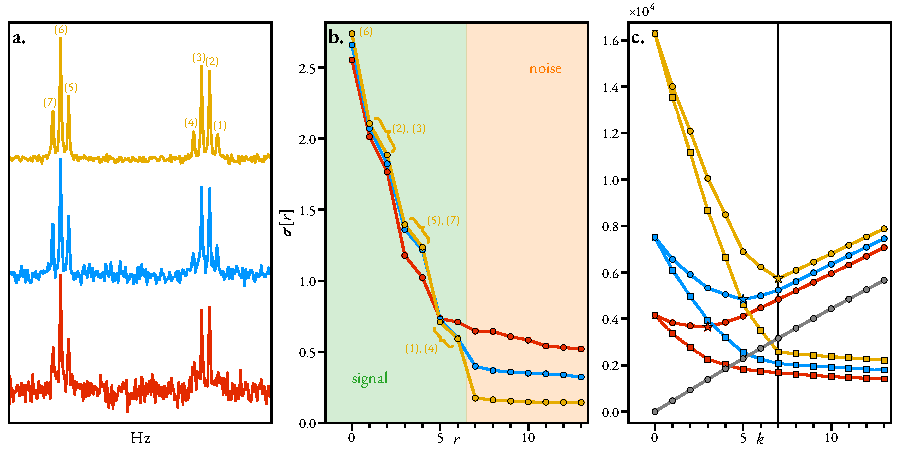
\includegraphics{mdl/mdl.pdf}
    \caption[
        An visualisation of the behaviour of the \acs{MDL} for three different
        \acsp{FID} comprising the same model, but with different noise variances.
    ]{
        An visualisation of the behaviour of the \acs{MDL} for three different
        \acsp{FID} comprising the same model, but with different noise
        variances. The model features 7 oscillators, comprising a 1:3:3:1 quartet
        structure and a 1:2:1 triplet structure. The three \acsp{SNR} used were
        \qty{20}{\deci\bel} (yellow), \qty{12}{\deci\bel} (blue), and
        \qty{7}{\deci\bel} (red). The \acsp{FID} were generated with $\None =
        256$.
        \textbf{a.} Spectra of the three \acsp{FID}.
        \textbf{b.} The values of the 14 most significant singular values
        associated with the Hankel matrix $\symbf{H}_{\symbf{Y}}$ (the pencil
        parameter $\Lone$ was set to $\lfloor \nicefrac{\None}{3} \rfloor =
        85$).
        \textbf{c.} Square points with dotted lines: The value of
        $-\ln \mathcal{L}$ at the \ac{MLE}, given by the negative of
        \eqref{eq:wax-pdf}.
        Grey line: the penalty component of the \ac{MDL}, given by the second
        term in \eqref{eq:mdl}.
        Circular points with solid lines: the \ac{MDL}.
        Stars denote the minimum of the \ac{MDL}. The \qty{20}{\deci\bel}
        signal is correctly deemed to have a model order of 7, while the other
        two are underestimated (predicted models orders are 5 and 2 for the
        \qty{12}{\deci\bel} and \qty{7}{\deci\bel} \acsp{FID}, respectively).
    }
    \label{fig:mdl}
\end{figure}
